\documentclass{ctexart}
\usepackage{morelull}
\usepackage{graphicx}
% \usepackage{amsmath}

\title{流体力学入门之张量分析}
\author{陈俊霖}
\date{\today}

\begin{document}

\maketitle
\tableofcontents

\begin{abstract}
本文是物理海洋学新兵蛋子在过去一个多月头晕目眩总结出来的“糟糠之作”,主要用途是用于应付我导(误),并顺便给自己做个全面的总结,以后可以常回头看看,常读常新。排版之丑,格式之混乱,举世罕见,见笑于大方之家。
本文主要内容包括:张量的基本概念,指标表示法,求和约定,克罗内克尔符号,置换符号和场论初步等等;同时,对于一些比较难以理解并且我也不懂的知识,比如说坐标变化和上下指标等内容,我就只能选择性忽略了,但是这并不影响你构建一个完整的知识体系。

\end{abstract}

\section{参考资料}
    \begin{itemize}
    \item{香港科技大学MATH4326课程的Lecture-2-1,Lecture-2-2和tutorial1}
    \item{吴望一《流体力学(上册)》第一章}
    \item{浙江大学刘海江《计算流体力学》2020-09-29第6-9节}
    \item{李东岳《无痛苦N-S方程笔记》}
    \item{《物理学中的张量分析》}
    \item{《张量分析》黄克智}
    \item{西安交通大学研究生课程张量分析及其工程应用课件}
    \item{Vector Calculus_Authors: Matthews, Paul C}
    \end{itemize}
    
\section{为何要学习张量}
最美的故事需要用最美的语言,而张量就是力学的语言,尤其是在连续介质力学中各项基本方程中的基本量——应力与应变都是张量,\代码{张量分析}实在是不能错过的有利数学工具。接下来,让我们一起出发,去探寻张量的秘密。

\section{引子}
\par
我们先来看看看一组解析形式的N-S方程,左边第一项为局地变化项,左边二至四项为迁移变化项,右边第一项为压强梯度力项,右边第二项为分子黏性力项,其中\代码{${\mu}$}是动力学黏性系数。

 $$ \frac{\partial u}{\partial t}+u \frac{\partial u}{\partial x}+v \frac{\partial u}{\partial y}+w \frac{\partial u}{\partial z}=-\frac{1}{\rho} \frac{\partial p}{\partial x}+\frac{\mu}{\rho} \Delta u $$
 
 $$ \frac{\partial v}{\partial t}+u \frac{\partial v}{\partial x}+v \frac{\partial v}{\partial y}+w \frac{\partial v}{\partial z}=-\frac{1}{\rho} \frac{\partial p}{\partial y}+\frac{\mu}{\rho} \Delta v $$
 $$ \frac{\partial w}{\partial t}+u \frac{\partial w}{\partial x}+v \frac{\partial w}{\partial y}+w \frac{\partial w}{\partial z}=-\frac{1}{\rho} \frac{\partial p}{\partial z}+\frac{\mu}{\rho} \Delta w $$
 
 是不是感觉太多,太复杂,胳膊有点酸,没有关系,我们高中好像学过矢量,我们知道用速度矢量$\vec{u}$的三个速度分量分别是$u,v,w$,那么可以用矢量形式将这三个公式“一网打尽”:
 
 $$\frac{\partial \vec{u}}{\partial t}+(\vec{u} \cdot \nabla) \vec{u}=-\frac{1}{\rho} \nabla \p+\frac{\mu}{\rho} \Delta \vec{u} $$
 
 同样地,我们可以使用张量的形式改写此方程,得到的表达式如下:
 $$ \frac{\partial u_{i}}{\partial t}+u_{j} \frac{\partial u_{i}}{\partial x_{j}}=-\frac{1}{\rho} \frac{\partial p}{\partial x_{i}}+\frac{\mu}{\rho} \frac{\partial^{2} u_{i}}{\partial x_{j}^{2}} $$
 \par
 需要特别说明的是,这里张量表达式中的$i$,$j$和以往直角坐标系中只表示一个特定方向的量有所不同,这里的$i$,$j$表示三个方向求和后的结果,这将在3.3中展开说明。
 
 我们可以发现,使用矢量或者张量表达式,具有形式简便、书写优美等特点,克服了解析表达式中的冗
 长的缺点。但是解析形式使用上理解起来是比较方便的,感觉张量形式就像是给物理或几何量加了一把钥匙,所以我们还将进一步学习张量中的具体定义、性质以及运算技巧。有细心的朋友会发现,好像张量形式的表达式和矢量表达式中的各项略有区别,增加了一些下标,这些下标具有有何含义,在运算中又会发生什么样的作用呢?让我们拭目以待吧!


\subsection{张量定义}
    首先,我们要明白什么是张量,我们之前学习的很多物理概念,在张量中又是如何表示的呢?有些教科书用的是坐标变化的方法,有的教科书将张量看成一种表示方法,有的教科书没有直接给出定义、而是从标量和矢量开始讲起,进而引申到张量。林林总总,其实只要自己看得懂就好。\par
    维基百科告诉我们,张量是一个可用来表示在一些矢量、标量和其他张量之间的线性关系的多线性函数。简单来讲,就是在三维空间和选定的坐标系中,需要同时用$3^n$个量来定义的量,我们称之为n阶张量,如果选定的时笛卡尔坐标系(直角坐标系),我们就称之为笛卡尔张量。\par
    大部分情况下,只需要能够熟练运用二阶笛卡尔张量的部分知识就可以了。
\begin{提示}
    \begin{itemize}
    \item{零阶张量:也即标量,只有大小、没有方向,如温度T,密度$\rho$;描述 0 阶张量所需要的量的个数为 $3^0=1$}
    \item{一阶张量:也即矢量,如位移矢量$\vec{r}$、加速度矢量$\vec{a}$;在三维空间中有3个分量}
    \item{二阶张量:在三维空间中有9个分量,如应力张量是二阶张量,在三维空间中的9个分量,包括3个应力张量以及6个剪切应力(剪切应力总是成对出现);}
    \item{n阶张量:在实际问题中出现较少;比较常见的是3阶张量——置换符号$\varepsilon $,描述其需要的量的个数为$3^3=27$}
    \end{itemize}
\end{提示}

\subsection{指标表示法}
\begin{提醒}
    在直角坐标系中,任一矢量可以写成:
    $$ \vec{a}={a}_{x}\vec{i}+{a}_{y}\vec{j}+{a}_{z}\vec{k} $$
    其中,${a}_{x}$、${a}_{y}$和${a}_{z}$是$\vec{a}$在x、y、z坐标下上的分量,$\vec{i}$、$\vec{j}$和$\vec{k}$是坐标x、y和z方向上的单位长度矢量,又称为坐标基矢量。
    这是我们最最常见的矢量表示方法,为了便于使用张量标记并在不同基矢量下进行转换和简单的运算,我们又如下约定和转换:
    $$
    \left\{\begin{array}{r}
    (x,y,z)=(x_1,x_2,x_3) \\
    (\vec{i}, \vec{j}, \vec{k})=\left(\boldsymbol{e_{1}}, \boldsymbol{e_{2}},\boldsymbol{e_{3}}\right) \\
    \left(a_{x}, a_{y}, a_{z}\right)=\left(a_{1}, a_{2}, a_{3}\right) \\
    \vec{a}=a_{1} \boldsymbol{e_{1}}+a_{2} \boldsymbol{e_{2}}+a_{3} \boldsymbol{e_{3}}
    \end{array}\right.
    $$
    
\end{提醒}

\subsection{求和约定}
\begin{注意}
    再进一步简化,也可以把矢量$\vec{a}$表示成
    $$ \vec{a} = \sum_{i=1}^{3}a_i \boldsymbol{e_i}= a_i \boldsymbol{e_i}$$
    \par
    这种表示矢量的方法叫做指标表示法,指标表示法一般有上角标和下角标,分别表示逆变矢量和协变矢量,但是通常来讲不用学习如此深入。细心的同学会发现,上式最后一项和中间一项相比,省去了求和符号,这是我们的约定,称为\代码{求和约定},通常也叫做\代码{爱因斯坦约定}。其内容是:某一指标,在一项中出现两次,则表示该指标取遍i=1,2,3的所有值(遍历求和)。
    \par
    “妈妈再也不用担心我胳膊酸痛啦”!!!
    \par
    再来几点补充说明:\\
    (1)遍历求和的指标称为哑指标;\\
    (2)没有求和的指标称为自由标;\\
    (3)哑指标就意味着求和,其下标的符号没有实际意义,因此$a_i\boldsymbol{e_i}$与$a_j\boldsymbol{e_j}$含义是相同的;\\
    (4)一项中可以同时出现自由标和哑指标;\\
    (5)当两个和式相乘时,哑指标不能重复,如果这两个和式原来采用的哑指标相同,则在将他们相乘时,应该讲其中一个哑指标换成其他符号。(这个在下一节讲张量运算法则时候尤其实用,我以前就搞不懂这个,吃了很多亏)
    
\end{注意}
    还是这个公式(张量形式的不可压缩流体的Navier-Stokes方程如下):
    $$
    \frac{\partial u_{i}}{\partial t}+u_{j} \frac{\partial u_{i}}{\partial x_{j}}=-\frac{1}{\rho} \frac{\partial p}{\partial x_{i}}+\frac{\mu}{\rho} \frac{\partial^{2} u_{i}}{\partial x_{j}^{2}}+f_{i}
    $$
    \par
    我们如何将其再次转回解析形式,我们应该如何分析其中的哑指标和自由标呢?
    首先,我们很容易知道,上式中i为自由标,j为哑指标(同一项中出现两次),所以就可以根据求和约定对下标j进行展开,写成三项求和的形式,如下:
    $$
    \frac{\partial u_{i}}{\partial t}+u_{1} \frac{\partial u_{i}}{\partial x_{1}}+u_{2} \frac{\partial u_{i}}{\partial x_{2}}+u_{3} \frac{\partial u_{i}}{\partial x_{3}}
    =-\frac{1}{\rho} \frac{\partial p}{\partial x_{i}}+\frac{\mu}{\rho}\left(\frac{\partial^{2} u_{i}}{\partial x_{1}^{2}}+\frac{\partial^{2} u_{i}}{\partial x_{2}^{2}}+\frac{\partial^{2} u_{i}}{\partial x_{3}^{2}}\right)+f_{i}
    $$
    \par
    这个理解起来比较容易,接下来我们需要对自由标i下手,自由标不需要进行求和,就依次展开为三项即可,好的,接下来又要写断胳膊了:
    $$
    \left\{\begin{array}{r}
    \frac{\partial u_{1}}{\partial t}+u_{1} \frac{\partial u_{1}}{\partial x_{1}}+u_{2} \frac{\partial u_{1}}{\partial x_{2}}+u_{3} \frac{\partial u_{1}}{\partial x_{3}}=-\frac{1}{\rho} \frac{\partial p}{\partial x_{1}}+\frac{\mu}{\rho}\left(\frac{\partial^{2} u_{1}}{\partial x_{1}^{2}}+\frac{\partial^{2} u_{1}}{\partial x_{2}^{2}}+\frac{\partial^{2} u_{1}}{\partial x_{1}^{2}}\right)+f_{1} \\
    \frac{\partial u_{2}}{\partial t}+u_{1} \frac{\partial u_{2}}{\partial x_{1}}+u_{2} \frac{\partial u_{2}}{\partial x_{2}}+u_{3} \frac{\partial u_{2}}{\partial x_{3}}=-\frac{1}{\rho} \frac{\partial p}{\partial x_{2}}+\frac{\mu}{\rho}\left(\frac{\partial^{2} u_{2}}{\partial x_{1}^{2}}+\frac{\partial^{2} u_{2}}{\partial x_{2}^{2}}+\frac{\partial^{2} u_{2}}{\partial x_{3}^{2}}\right)+f_{2} \\
    \frac{\partial u_{3}}{\partial t}+u_{1} \frac{\partial u_{3}}{\partial x_{1}}+u_{2} \frac{\partial u_{3}}{\partial x_{2}}+u_{3} \frac{\partial u_{3}}{\partial x_{3}}=-\frac{1}{\rho} \frac{\partial p}{\partial x_{3}}+\frac{\mu}{\rho}\left(\frac{\partial^{2} u_{3}}{\partial x_{1}^{2}}+\frac{\partial^{2} u_{3}}{\partial x_{2}^{2}}+\frac{\partial^{2} u_{3}}{\partial x_{j}^{2}}\right)+f_{3}
    \end{array}\right.
    $$
    \par
    是不是感受到了满满的恶意,没事,我们还能再抢救一下,写成分量的形式,这个大家看上去就比较顺眼了:
    $$
    \left\{\begin{array}{r}
    \frac{\partial u}{\partial t}+u \frac{\partial u}{\partial x}+v \frac{\partial u}{\partial y}+w \frac{\partial u}{\partial z}=-\frac{1}{\rho} \frac{\partial p}{\partial x}+\frac{\mu}{\rho}\left(\frac{\partial^{2} u}{\partial x^{2}}+\frac{\partial^{2} u}{\partial y^{2}}+\frac{\partial^{2} u}{\partial z^{2}}\right)+f_{x} \\
    \frac{\partial v}{\partial t}+u \frac{\partial v}{\partial x}+v \frac{\partial v}{\partial y}+w \frac{\partial v}{\partial z}=-\frac{1}{\rho} \frac{\partial p}{\partial y}+\frac{\mu}{\rho}\left(\frac{\partial^{2} v}{\partial x^{2}}+\frac{\partial^{2} v}{\partial y^{2}}+\frac{\partial^{2} v}{\partial z^{2}}\right)+f_{y} \\
    \frac{\partial w}{\partial t}+u \frac{\partial w}{\partial x}+v \frac{\partial w}{\partial y}+w \frac{\partial w}{\partial z}=-\frac{1}{\rho} \frac{\partial p}{\partial z}+\frac{\mu}{\rho}\left(\frac{\partial^{2} w}{\partial x^{2}}+\frac{\partial^{2} w}{\partial y^{2}}+\frac{\partial^{2} w}{\partial z^{2}}\right)+f_{z}
    \end{array}\right.
    $$

\section{张量运算}
     知道了张量的具体定义之后,我们还需要学习一些在张量理论中可以帮助我们进行运算的一些重要符号。
\subsection{克罗内克尔符号}
    \begin{定义}{Kronecker}{Kronecker}
    克罗内克尔符号$\delta_{ij}$,它定义为\\
    $$
    \boldsymbol{{e}_{i}} \cdot \boldsymbol{{e}_{j}}=\delta_{ij}=\left\{\begin{array}{ll}
    1, & i=j  \\
    0, & i \neq j 
    \end{array}\right.
    $$
    \end{定义}
    显而易见地,$\delta_{ij}$应该满足交换律,也即$\delta_{ij}=\delta_{ji}$。再结合上一节中有关自由标和哑指标的概念,我们可以得到一些有意思的结论:
    $$ \delta_{ii} = \delta_{jj} =\delta_{11} +\delta_{22} +\delta_{33}=3 $$ 
    $$ \delta_{ii}\delta_{jj}=(\delta_{11} +\delta_{22} +\delta_{33})(\delta_{11} +\delta_{22} +\delta_{33})=\delta_{11}\delta_{11}+\delta_{22}\delta_{22}+\delta_{33}\delta_{33}=3 $$
    $$
    \delta_{ij}A_{j}=\delta_{i1}A_1+\delta_{i2}A_2+\delta{i3}A_3=\delta_{11} A_{1}+\delta_{22} A_{2}+\delta_{33} A_{3}=\left(\begin{array}{c}
    A_{1} \\
    A_{2} \\
    A_{3}
    \end{array}\right)=A_{i}
    $$
    $$ \delta_{ij}\delta_{kj}=\delta_{ik} $$
    \par
    对于任意的矢量$\boldsymbol{a}$和$\boldsymbol{b}$,使用指标表示法表示方式如下:
    $$
    \left\{\begin{array}{l}
    \boldsymbol{a}=a_{1} e_{1}+a_{2} \boldsymbol{e}_{2}+a_{3} \boldsymbol{e}_{3}=\sum_{i=1}^{3} a_{i} \boldsymbol{e}_{i}=a_{i} \boldsymbol{e}_{i} \\
    \boldsymbol{b}=b_{1} \boldsymbol{e}_{1}+b_{2} \boldsymbol{e}_{2}+b_{3} \boldsymbol{e}_{3}=\sum_{i=1}^{3} b_{i} \boldsymbol{e}_{i}=b_{i} \boldsymbol{e}_{i}
    \end{array}\right.
    $$
    \par
    矢量$\boldsymbol{a}$和$\boldsymbol{b}$的内积计算结果如下:(注意:两个和式相乘时,哑指标不能重复)
    $$
    \boldsymbol{a} \cdot \boldsymbol{b}=a_{i} \boldsymbol{e}_{i} \cdot b_{j} \boldsymbol{e}_{j}=a_{i}b_{j}\delta_{ij}=a_{i}b_{i}=a_{j}b_{j}
    $$

\subsection{置换符号}

     \begin{定义}{置换符号}{置换符号}
    我们先来看一组基矢量的叉乘:
    $$
    \left\{\begin{array}{ll}
     \boldsymbol{e_{1}} \times \boldsymbol{e_{2}}=-\boldsymbol{e_{2}} \times \boldsymbol{e_{1}}=\boldsymbol{e_{3}} \\
    \boldsymbol{e_{2}} \times \boldsymbol{e_{3}}=- \boldsymbol{e_{3}}\times \boldsymbol{e_{2}}=\boldsymbol{e_{1}} \\
     \boldsymbol{e_{3}} \times \boldsymbol{e_{1}}=-\boldsymbol{e_{1}} \times \boldsymbol{e_{3}}=\boldsymbol{e_{1}}
     \end{array}\right.
     $$
     \par
     当然,一个矢量还可以和自己相乘:
     $$
     \boldsymbol{e}_{i} \times \boldsymbol{e}_{j}=0 \quad(i=j)
     $$\par
     有没有什么符号可以将以上这些公式一网打尽呢?
     有点,那就是\代码{置换符号}!
     \par
     置换符号$\varepsilon $,我们又把它称为排列符号,它的定义如下
     $$
     \varepsilon_{i j k}=\left\{\begin{array}{ll}
     1, & \text { i,j,k 为偶排列。如 }(1,2,3),(2,3,1),(3,1,2) \text { 等 } \\
    -1, & \text { i,j,k 为奇排列。如 }(2,1,3),(1,3,2),(3,2,1) \text { 等 } \\
    0, & \text { i,j,k 不成排列。如 }(1,1,2),(1,1,1) \text { 等 }
     \end{array}\right.
    $$
    \par
    插一句(回忆一下线性代数的知识):偶排列和奇排列的定义如下:逆序数为偶数的排列称为偶排列;逆序数为奇数的排列称为奇排列。\代码{举个栗子},初始排列123变为231,可以通过三个逆序对换得到:首先交换1和3的位置,得到321;然后交换2和3,得到231,因此(2,3,1)是一个偶排列,逆序数为2。(或者大家可以看看下面的示意图,顺时针的就是偶排列,逆时针的就是奇排列。)
    \begin{center}
        1 \quad
     \end{center}
    \begin{center}
      $  \nearrow \quad \nwarrow $
     \end{center}
     \begin{center}
       $3 \longleftarrow \quad  2 $
     \end{center}
    \par
    利用置换符号$\varepsilon$,我们可以简化矢量叉乘的式子
    $$ 
    \boldsymbol{e_i} \times \boldsymbol{e_j}=\varepsilon_{i j k}\boldsymbol{e_k}
    $$
    \end{定义}
    我们可以验证一下,当i=j时候,上式右边为0,当$i \neq j$的时候,上式右边和式三项只有当$k \neq i$且$k \neq j$的一项不为0,因此使用置换公式可以完美解决坐标基矢的叉乘问题。
    同样地,我们希望可以计算任意矢量$\boldsymbol{a}$和$\boldsymbol{b}$的叉乘:(看上去有27项,但是使用置换符号之后你会发现一下子就只剩下6项)
    $$
    \begin{aligned}
    \boldsymbol{a} \times \boldsymbol{b}&=\sum_{i=1}^{3} \sum_{j=1}^{3} \sum_{k=1}^{3} \varepsilon_{i j k} a_{i} b_{j} \boldsymbol{e}_{k} 
      \\
      &=\varepsilon_{i j k} a_{i} b_{j} \boldsymbol{e}_{k} 
      \\
       &=\varepsilon_{123}a_{1}b_{2}\boldsymbol{e}_{3}+\varepsilon_{132}a_{1}b_{3}\boldsymbol{e}_{2}+\varepsilon_{231}a_{2}b_{3}\boldsymbol{e}_{1}+\varepsilon_{213}a_{2}b_{1}\boldsymbol{e}_{3}+\varepsilon_{312}a_{3}b_{1}\boldsymbol{e}_{2}+\varepsilon_{321}a_{3}b_{2}\boldsymbol{e}_{1} 
       \\
       &= (a_{2}b_{3}-a_{3}b_{2})\boldsymbol{e}_{1}+(a_{3}b_{1}-a_{1}b_{3})\boldsymbol{e}_{2}+(a_{1}b_{2}-a_{2}b_{1})\boldsymbol{e}_{3}
       \\
       &=\left|\begin{array}{lll}
      \boldsymbol{e}_{1} & \boldsymbol{e}_{2} & \boldsymbol{e}_{3} \\
       a_{1} & a_{2} & a_{3} \\
       b_{1} & b_{2} & b_{3}
      \end{array}\right|
    \end{aligned}
   
     $$
     
     \par
     我们还能在以下场景中使用置换符号$\varepsilon$,比如说计算三阶行列式:(还是在复习线性代数的知识)
     $$
    \left|\begin{array}{lll}
    a_{1} & a_{2} & a_{3} \\
    b_{1} & b_{2} & b_{3} \\
    c_{1} & c_{2} & c_{3}
    \end{array}\right|=\sum_{i, j, k}^{3} \varepsilon_{i j k} a_{i} b_{j} c_{k}
    $$
    
    
\subsection{三矢量的连乘积}
    在知道了克罗内克尔符号和置换符号之后,我发现我还是只能解决两个矢量点乘和叉乘的问题,而这是远远不够的,我们还需要把上面两节的知识结合起来,学习如何解决三矢量的连乘积问题,这个会在今后的很多学习场景中遇到,要解决这个问题本质来只是简单地数学变化,并不需要害怕。同时,我会在这一节中介绍三矢量连乘积的数学图像,有助于加深你们对于三矢量的连乘积的理解。三个矢量$ \boldsymbol{a}$,$ \boldsymbol{b}$和$\boldsymbol{c}$的连乘有两种,一种是$\boldsymbol{a} \cdot( \boldsymbol{b} \times \boldsymbol{c})$,另外一种是$\boldsymbol{a} \times (\boldsymbol{b} \times \boldsymbol{c})$。\\
    我们先来介绍前一种(有些书上称之为“混合积”)——
    $$
    \boldsymbol{a} \cdot (\boldsymbol{b} \times \boldsymbol{c})=a_{i}(\boldsymbol{b} \times \boldsymbol{c})_{i}=a_{i} \varepsilon_{i j k} b_{j} c_{k}=\varepsilon_{i j k} a_{i} b_{j} c_{k}=\left|\begin{array}{lll}
    a_{1} & a_{2} & a_{3} \\
    b_{1} & b_{2} & b_{3} \\
    c_{1} & c_{2} & c_{3}
    \end{array}\right|
    $$
    \par
    最后我们可以得到一个行列式的形式,容易知道,将这一行列式中的三行顺序轮换,取值不变,因此我们可以得到:
    $$
    \boldsymbol{a} \cdot (\boldsymbol{b} \times \boldsymbol{c})=\boldsymbol{b} \cdot (\boldsymbol{c} \times \boldsymbol{a})=\boldsymbol{c} \cdot (\boldsymbol{a} \times \boldsymbol{b})
    $$
    \par
    下面我们来看看这个公式的数学图像,首先$\boldsymbol{s}=\boldsymbol{b} \times \boldsymbol{c}$是一个垂直于$(\boldsymbol{b},\boldsymbol{c})$平面的矢量,其长度为$s=bc \sin\theta_{bc}$——等于两个矢量$\boldsymbol{b}$和$\boldsymbol{c}$所围成的平行四边形的面积。而$\boldsymbol{a} \cdot \boldsymbol{s}=(a \cos\theta_{as})_{S}$等于由$ \boldsymbol{a}$,$ \boldsymbol{b}$和$\boldsymbol{c}$形成的平行六面体的高$a \cos\theta_{as}$乘以底面积s,因此等于这一平行六面体的体积。\\
    三个矢量的连叉乘的计算——$\boldsymbol{a} \times (\boldsymbol{b} \times \boldsymbol{c})$稍微复杂一点,用前面两节的内容我们还没法进行计算,我们将在下一节中介绍一有利的武器,它将帮助我们解决这一问题。
\subsection{$ \varepsilon $ -$ \delta $恒等式}
我们在4.1和4.2中分别学习了$ \delta $、$ \varepsilon $,这是进行张量计算的有利武器,理解这两个算子的关系能更加有利于我们进行张量计算。由4.3中的知识,我们可以得到——$\epsilon_{i j k}=\boldsymbol{e}_{i} \cdot (\boldsymbol{e}_{j} \times \boldsymbol{e}_{k})$。
$$
\varepsilon_{i j k}=\boldsymbol{e}_{i} \cdot\left(\boldsymbol{e}_{j} \times \boldsymbol{e}_{k}}\right)=\left|\begin{array}{ccc}
\boldsymbol{e}_{i} \cdot \boldsymbol{e}_{1} & \boldsymbol{e}_{i} \cdot \boldsymbol{e}_{2} & \boldsymbol{e}_{i} \cdot \boldsymbol{e}_{3} \\
\boldsymbol{e}_{j} \cdot \boldsymbol{e}_{1} & \boldsymbol{e}_{j} \cdot \boldsymbol{e}_{2} & \boldsymbol{e}_{j} \cdot \boldsymbol{e}_{3} \\
\boldsymbol{e}_{k} \cdot \boldsymbol{e}_{1} & \boldsymbol{e}_{k} \cdot \boldsymbol{e}_{2} & \boldsymbol{e}_{k} \cdot \boldsymbol{e}_{3}
\end{array}\right|=\left|\begin{array}{ccc}
\delta_{i 1} & \delta_{i 2} & \delta_{i 3} \\
\delta_{j 1} & \delta_{j 2} & \delta_{j 3} \\
\delta_{k 1} & \delta_{k 2} & \delta_{k 3}
\end{array}\right|
$$
\par
所以,我们有
$$
\begin{aligned}
\varepsilon_{i q k} \varepsilon_{p q r} &=\left|\begin{array}{lll}
\delta_{i 1} & \delta_{i 2} & \delta_{i 3} \\
\delta_{j 1} & \delta_{j 2} & \delta_{j 3} \\
\delta_{k 1} & \delta_{k 2} & \delta_{k 3}
\end{array} \| \begin{array}{lll}
\delta_{p 1} & \delta_{p 2} & \delta_{p 3} \\
\delta_{q 1} & \delta_{q 2} & \delta_{q 3} \\
\delta_{r 1} & \delta_{r 2} & \delta_{r 3}
\end{array}\right| \\
&=\left|\begin{array}{lll}
\delta_{i p} & \delta_{i q} & \delta_{i r} \\
\delta_{j p} & \delta_{j q} & \delta_{j r} \\
\delta_{k p} & \delta_{k q} & \delta_{k r}
\end{array}\right|
\end{aligned}
$$
\par
这个公式过于复杂,我们只需要记住其中一些有关$\varepsilon$的一些有用的结论就可以了:

\begin{结论}{}{}
   (1)其中有一个下标相同时,如k=r时——
   $$
\begin{aligned}
\varepsilon_{i j k} \varepsilon_{p q k} &=\left|\begin{array}{lll}
\delta_{i p} & \delta_{i q} & \delta_{i k} \\
\delta_{j p} & \delta_{j q} & \delta_{j k} \\
\delta_{k p} & \delta_{k q} & \delta_{k k}
\end{array}\right| \\
&=3\left(\delta_{i p} \delta_{j q}-\delta_{i q} \delta_{j p}\right)-\delta_{k q}\left(\delta_{i p} \delta_{j k}-\delta_{i k} \delta_{j p}\right)-\delta_{k p}\left(\delta_{i k} \delta_{j p}-\delta_{i q} \delta_{j k}\right) \\
&=\delta_{i p} \delta_{j q}-\delta_{i q} \delta_{j p} \\
&=\left|\begin{array}{ll}
\delta_{i p} & \delta_{i q} \\
\delta_{j p} & \delta_{j p}
\end{array}\right|
\end{aligned}
$$
\par
   (2)其中有两个下标相同时,例如k=r,q=j时——
   $$
\varepsilon_{i j k} \varepsilon_{p j k}=\left|\begin{array}{ll}
\delta_{i p} & \delta_{i j} \\
\delta_{j p} & \delta_{j j}
\end{array}\right|=3 \delta_{i p}-\delta_{i j} \delta_{j p}=2 \delta_{i p}
$$
\par
   (3)三个下标都相等时——
   $$
   \varepsilon_{i j k} \varepsilon_{i j k} =2\delta{ii}=6
   $$
\end{结论}
    接下来,我们将使用此恒等式,计算三矢量连叉乘$\boldsymbol{a} \times (\boldsymbol{b} \times \boldsymbol{c})$的结果。(有些书上称之为“三重积”)
    $$
    \begin{aligned}
    \boldsymbol{a} \times(\boldsymbol{b} \times \boldsymbol{c})=& a_{q} \boldsymbol{e}_{q}} \times \varepsilon_{i j k} b_{i} c_{j} \boldsymbol{e}_{k} \\
    &=\varepsilon_{i j k} \varepsilon_{p q k} a_{q} b_{i} c_{j} \boldsymbol{e}_{p} \\
    &=\left(\delta_{i p} \delta_{j q}-\delta_{i q} \delta_{j p}\right) a_{q} b_{i} c_{j}  \boldsymbol{e}_{p} \\
     &={a}_{q}{c}_{j} \delta_{j q}{b}_{i}(\boldsymbol{e}_{i} \cdot \boldsymbol{e}_{p} \cdot \boldsymbol{e}_{p})-{a}_{q}{b}_{i} \delta_{i q}{c}_{j}(\boldsymbol{e}_{j} \cdot \boldsymbol{e}_{p} \cdot \boldsymbol{e}_{p})\\
    &=(\boldsymbol{a} \cdot \boldsymbol{c}) ({b}_{i} \boldsymbol{e}_{i})-(\boldsymbol{a} \cdot \boldsymbol{b})({c}_{j} \boldsymbol{e}_{j}) \\
    &=(\boldsymbol{a} \cdot \boldsymbol{c}) \boldsymbol{b}-(\boldsymbol{a} \cdot \boldsymbol{b}) \boldsymbol{c}
    \end{aligned}
    $$
    \par
    使用这种方法不难计算更多的矢量连乘积。一下是一些可能用到的一些计算公式:
    


\subsection{总结} 
     \begin{结论}{}{}
    总而言之,言而总之,这两个符号,一个针对矢量点乘,一个针对矢量叉乘,还有一个公式能把他们连接起来,那么基本上所有的矢量、笛卡尔张量的计算都是基于这一节归纳的内容的基础上的,包括我们第五节场论中出现的比较复杂的算子和公式。纲举自然目张,学习其他知识也是这样子的!
     \end{结论}

\newpage
\section{场论}
      设在空间中的某个区域内定义标量函数或者矢量函数,则称定义在此空间区域内的函数为场——如果研究的是标量函数则称此场为\代码{标量场},如果研究的时矢量函数,则称此场为\代码{矢量场}。\par
      其实就仨事,梯度、散度和旋度。\par
      
      我们首先来看思考一下,我们如何在空间中表示一个标量场或者矢量场?

\subsection{场的几何表示}
      用几何方法表示一个场有助于直观地理解问题,并且具有实际意义。
      首先我们来研究标量场$\psi(\vec{r},t)$的几何表示,就两个量,一个是位置矢量,一个是时间变量。首先,对于定常场(稳定场)来说,场中各物理量不随时间变化,那么只需要研究$\psi(\vec{r})$即可。对于不稳定场,如果在每一个时刻,场的几何表示都已经知道了,则整个场的几何表示也就知道了。
      \par
      因此,只须选取任意一固定时刻,研究场$\psi(\vec{r},t_0)$的几何表示。\par
      令
      $$
      \psi(\vec{r},t_0)=\text{constant}=\psi_0
      $$
      \par
      得到与之对应的曲面称之为等位面,在等位面上$\psi$的取值处处相等,取一系列不同的$\psi_0$值,我们可以得到空间中一组与之对应的等位面,于是整个标量场为划分为很多不同区域。\par
      作出等位面之后,我们就可以从等位面的相互位置,它的疏密程度看出标量场的变化情况。
      \par
      矢量场的几何表示较标量场要复杂一些,因为矢量场既有大小,又有方向,需要分别对其大小和方向做几何表示。由于矢量场大小是一个标量,所以可以用上面等位面的概念来几何地表示它。
      \par
      至于矢量的方向,我们可以引入矢量线对其进行几何表示。
      \begin{定义}{矢量线}
      矢矢量线就是这样的曲线,在曲线上每一点出,曲线都和该点对应的矢量($\vec{A}$)相切。\par
      \代码{最经典的矢量线就是流线,流线的切线方向就是流速的方向。}
      设$\vec{r}$是矢量线的切线方向,则根据矢量线的定义,我们有
      $$
       \vec{A} \times d\vec{r}=0\\
      $$
      \par
      展开,得到:
      $$
\begin{array}{l}
\vec{A} \times d \vec{r}=\varepsilon_{i j k} A_{j} d r_{k}=\left(A_{2} d r_{3}-A_{3} d r_{2}\right) \boldsymbol{e}_{1}+\left(A_{3} d r_{1}-A_{1} d r_{3}\right) \boldsymbol{e_{2}}+\left(A_{1} d r_{2}-A_{2} d r_{1}\right) \boldsymbol{e}_{3}=0
\end{array}
$$
\par
因此,写成直角坐标分量形式的微分方程如下——
$$
\frac{d_{x}}{A_{x}}=\frac{d_{y}}{A_{y}}=\frac{d_{z}}{A_{z}}
$$
\par
有了矢量线之后,场内的每一点的矢量方向就可由矢量线的切线方向给出;同时,我们也可以从矢量线的疏密程度来估计矢量在各点的大小。
\end{定义}
在知道了如何用几何方法描述一个场之后,我们需要去研究场内各种物理量的变化情况。这也是学习的基本逻辑,首先知道是什么,然后知道怎么样。
\subsection{微分算子}
在开始介绍梯度、散度、旋度之前,我们要引入一个非常重要的微分运算子,实际上它在之前的章节中介绍N-S方程就曾经出现过,实际上应该是比较基础的知识,但是为了避免有人可能没有掌握这个知识点,我们先来打点铺垫,或者了解这个知识点的同学可以进行复习,对此可能会有深入的认识。
\par
首先是哈密顿算子,它的表达式是:
$$
\nabla =\vec{i} \frac{\partial}{\partial x}+\vec{j} \frac{\partial}{\partial y}+\vec{k} \frac{\partial}{\partial z} 
=\frac{\partial}{\partial x_{1}} \boldsymbol{e_{1}}+\frac{\partial}{\partial x_{2}} \boldsymbol{e_{2}}+\frac{\partial}{\partial x_{3}} \boldsymbol{e_{3}}=\frac{\partial}{\partial x_{i}} \boldsymbol{e_{i}}
$$
\par
这是一个具有矢量和微分双重性质的符号。首先,它是一个矢量,意味着在运算时候可以使用矢量代数和矢量分析中的所有法则;另一方面,它是一个微分算符,因此可以按照微分法则进行运算,但是要注意的是:\代码{这个微分算子只对算子$\nabla$右边的量发生微分作用,对于算子左边的量,算子$\nabla$对它不起作用}
\par
我们定义一个矢量$\vec{A}=A_j\boldsymbol{e_{j}}$和一个标量$\phi$。他们将在接下来的几节中扮演重要角色,以下是它们与哈密顿算子檫出美丽火花之后的结果:
$$
\nabla \cdot \vec{A} =\left(\frac{\partial}{\partial x_{i}} e_{i}\right) \cdot\left(A_{j} e_{j}\right)
=\frac{\partial A_{j}}{\partial x_{i}}\left(e_{i} \cdot e_{j}\right)=\delta_{i j} \frac{\partial A_{j}}{\partial x_{i}}=\frac{\partial A_{m}}{\partial x_{m}}
$$

$$
\nabla \phi = \frac{\partial \phi}{ \partial x_{i}} \boldsymbol{e_{i}}
$$

$$
\begin{aligned}
\nabla \times \vec{A} &=\left(\frac{\partial}{\partial x_{i}} \boldsymbol{e_{i}}\right) \times\left(A_{j} \boldsymbol{e_{j}}\right)=\varepsilon_{i j k} \frac{\partial A_{j}}{\partial x_{i}} \boldsymbol{e_{k}} \\
&=\left|\begin{array}{ccc}
\boldsymbol{e_{1}} & \boldsymbol{e_{2}} & \boldsymbol{e_{3}} \\
\frac{\partial}{\partial x_{1}} & \frac{\partial}{\partial x_{2}} & \frac{\partial}{\partial x_{3}} \\
A_{1} & A_{2} & A_{3}
\end{array}\right|
\end{aligned}
$$

\par
要特别注意的是,我们知道,哈密顿算子$\nabla$只对算子右边的量起作用,对算子左边的量不起作用,因此$\nabla \cdot \vec{A}$与$\vec{A} \cdot \nabla$意义是完全不同的。

$$
    \vec{A} \cdot \nabla =\left(A_{i} e_{i}\right) \cdot\left(\frac{\partial}{\partial x_{j}} e_{j}\right) 
   =\left(A_{i} \frac{\partial}{\partial x_{j}}\right)\left(e_{i} \cdot e_{j}\right) 
   =\partial i_{j} A_{i} \frac{\partial}{\partial x_{j}}=A_{m} \frac{\partial}{\partial    x_{m}}
$$

同时,我们还有二阶微分算子,它被定义为\代码{梯度场的散度场}。(在这里我们先按住这些奇奇怪怪的定义不表,在下面的章节中会有详细的定义,在这里出现不会影响你记忆一个人为规定的运算符)。简单来讲,就是如果你有一个二阶可微的实函数$\phi$,则$\phi$的拉普拉斯算子定义为:
$$
  \Delta \phi=\nabla^{2} \phi=\frac{\partial^{2} \phi}{\partial x^{2}}+\frac{\partial^{2} \phi}{\partial y^{2}}+\frac{\partial^{2} \phi}{\partial z^{2}}=\sum_{i=1}^{3} \frac{\partial^{2} \phi}{\partial x_{i}^{2}}=\frac{\partial^{2} \phi}{\partial x_{i}^{2}}
$$
\par
那为什么拉普拉斯算子这么重要?
因为标量函数的梯度往往是一种“驱动力”(或者叫“趋势”),而针对“驱动力”求散度就可以知道空间中“源”的分布。

\par
知道了这些算子,我们就可以简化一些花里胡哨的运算式子,并且得到一些比较有用的结论。



\subsection{梯度}
给定一标量场,我们想知道在标量场$\phi(\vec{r},t_0)$中,任一时刻每点领域内的函数变化。
我们引入梯度的概念,它可以衡量标量场不均匀性,标量场中某一点上的梯度指向标量场增长最快的方向,梯度的大小是这个最大的变化率。\par
\代码{由此可知,梯度应该是有大小,有方向的矢量场!}
$$
\operatorname{grad} \phi=\nabla \phi=\frac{\partial \phi}{\partial x} \vec{i}+\frac{\partial \phi}{\partial y} \vec{j}+\frac{\partial \phi}{\partial z} \vec{k} =\frac{\partial \phi}{\partial {x}_{i}} \boldsymbol{e_{i}}
$$
\par
标量场$\phi$中的每一点M处的梯度垂直于该点处的等值面,且指向函数$\phi(M)$增大的方向。\par
因此,在等值面上任一点的单位法向量$\vec{n}$可以通过该点的梯度来表示:
$$
\vec{n}=\frac{\nabla \phi}{\mid \nabla \phi \mid} 
$$

\subsection{散度}
\begin{定义}{散度}
   给给定矢量场$\vec{a}(\vec{r},t)$,在场内取一曲面S,它可以是封闭的也可以是不封闭的(曲面封闭,通常取外法线为正方向;若曲面不封闭,则可以约定取某一方向为正方向)。令$\vec{n}$表示S曲面上法线方向的单位矢量,$\vec{a}$表示M点上的矢量函数的值,定义面积矢量$d\vec{S}$是大小为dS方向为法线正方向的量。在曲线沿着其中有向曲面S某一侧的曲面积分:
   $$
  \Phi=\iint_{S} a_{n} d S=\iint_{S} \vec{a} \cdot \vec{n} d S=\int_{S} \vec{a} \cdot d \vec{S}
$$
\par
$\Phi$叫做矢量场$\vec{a}$向积分所沿一侧穿过曲面S的通量。其中,$a_{n}$代表矢量$\vec{a}$在法线方向的投影
$$
a_{n}=\vec{a} \cdot \vec{n}={a}_{x} \cos(\vec{n},x)+{a}_{y} \cos(\vec{n},y)+{a}_{z} \cos(\vec{n},z);
$$
\par 
\begin{center}
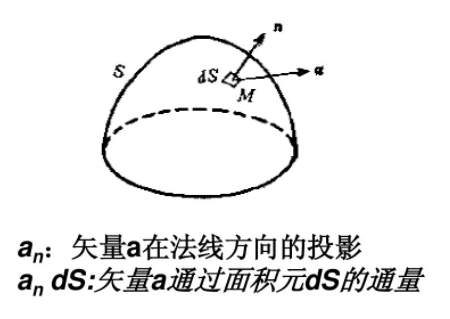
\includegraphics{divergence.png}
\end{center}

\par
  通量的极限就是\代码{散度}。令在场内任取一点M,以体积V包裹之,若V的界面是S,作矢量$\vec{a}$通过S面的通量,然后用体积V除之,令体积V向M点无限收缩,得到极限——
 
  $$
  \operatorname{div} \vec{a}=\lim _{V \rightarrow 0} \frac{\Phi}{V}=\lim _{V \rightarrow 0}\left(\frac{\partial a_{x}}{\partial x}+\frac{\partial a_{y}}{\partial y}+\frac{\partial a_{z}}{\partial z}\right)=\frac{\partial a_{x}}{\partial x}+\frac{\partial a_{y}}{\partial y}+\frac{\partial a_{z}}{\partial z}=\nabla \cdot \vec{a}=\frac{\partial a_{i}}{\partial x_{i}}=\delta_{i j} \frac{\partial a_{j}}{\partial x_{i}}
  $$
\end{定义}
因此,我们可以知道,散度表示矢量场中一点的通量对体积的变化率,也即是对单位体积而言矢量通过体积元界面的通量,称为该点处源的\代码{强度},\代码{散度场是标量场}。
\par
若矢量场$\vec{a}$中任意一点满足$\operatorname{div} \vec{a}=0$,则称矢量场$\vec{a}$为无源场。

\subsection{旋度}

\begin{定义}{旋度}
    给给定一矢量场$\vec{a}(\vec{r},t)$,M为场内一点,该点附近取无限小封闭曲线L,设张于L上的曲面为S,S的法线方向为$\vec{n}$。做矢量$\vec{a}$沿曲线L的环量并除以曲面面积S。令L向M点收缩,使得张于周线L的曲面矢量$\vec{S}=S_{\vec{n}$,其大小趋于零,方向趋于固定的方向$\vec{n}$,得到下列极限(如果极限存在的话),定义为矢量$\vec{a}$在$\vec{n}$方向的旋度(\代码{矢量的旋度为矢量}):
    $$
    \operatorname{rot}_{n} \vec{a}=\lim _{s \rightarrow 0} \frac{\oint_{L}^{}  \vec{a} \cdot d \vec{r}}{s}=(\operatorname{curl} \vec{a})_{n}
    $$
    
    \begin{center}
        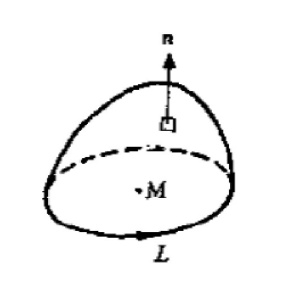
\includegraphics{rotation.png}
    \end{center}
    \par
    那可能大家会有疑问了,上式极限存在,它是否一定是某一矢量在n方向的投影?其实可以证明,如果矢量$\vec{a}$的三个分量具有连续一阶偏导数,则上式中的极限一定存在,且它的确是旋度在n方向的投影。
   
\end{定义}
     下面是证明过程:
    \par
    首先使用斯托克斯公式,我们有
    $$
    \begin{aligned}
        \oint_{L}^{} \vec{a} \cdot d \vec{r}
        &=\oint_{L}\left(a_{x} d x+a_{y} d y+a_{z} d z\right)
        \\
        &=\int_{S}[(\frac{\partial a_{z}}{\partial y}-\frac{\partial a_{y}}{\partial z}) \cos (n, x) +(\frac{\partial a_{x}}{\partial z}-\frac{\partial a_{z}}{\partial x}) \cos (n, y) 
        +\(\frac{\partial a_{y}}{\partial x}-\frac{\partial a_{x}}{\partial y}) \cos (n, z)] d S
       \end{aligned}
    $$
    \par
    利用中值公式,我们有
    $$
     \oint_{L} \vec{a} \cdot d \vec{r}=\operatorname{S}[(\frac{\partial a_{z}}{\partial y}-\frac{\partial a_{y}}{\partial z}) \cos (n, x) 
     +(\frac{\partial a_{x}}{\partial z}-\frac{\partial a_{z}}{\partial x}) \cos (n, y)+(\frac{\partial a_{y}}{\partial x}-\frac{\partial a_{x}}{\partial y}) \cos (n, z)]_{Q}
    $$
    \par
    其中,$Q$是曲面$S$上的某一点,将上式带入旋度公式$\operatorname{rot} _{n} \vec{a}$,我们有
    $$
    \begin{aligned}
    \operatorname{rot} _{n} \vec{a}=\lim _{s \rightarrow 0} \frac{\oint_{L} \vec{a} \cdot d \vec{r}}{s}=&\left(\frac{\partial a_{z}}{\partial y}-\frac{\partial a_{y}}{\partial z}\right) \cos (n, x) \\
    &+\left(\frac{\partial a_{x}}{\partial z}-\frac{\partial a_{z}}{\partial x}\right) \cos (n, y) \\
    &+\left(\frac{\partial a_{y}}{\partial x}-\frac{\partial a_{x}}{\partial y}\right) \cos (n, z)
    \end{aligned}
    $$
    \par
    将旋度$\operatorname{rot} _{n} \vec{a}$在直角坐标系中进行分解:
    $$
     \operatorname{rot} _{n} \vec{a} =  (\operatorname{rot} _{n} \vec{a})_{x} \cos(n,x) +(\operatorname{rot} _{n} \vec{a})_{y} \cos(n,y) +(\operatorname{rot} _{n} \vec{a})_{z} \cos(n,z)
    $$
    \par
    因为方向$n$是固定的,推出
    $$
    \left\{\begin{array}{l}
    \operatorname{rot}_{x} \vec{a}=\frac{\partial a_{z}}{\partial y}-\frac{\partial a_{y}}{\partial z} \\
    \operatorname{rot}_{y} \vec{a}=\frac{\partial a_{x}}{\partial z}-\frac{\partial a_{z}}{\partial x} \\
    \operatorname{rot}_{z} \vec{a}=\frac{\partial a_{y}}{\partial x}-\frac{\partial a_{x}}{\partial y}
    \end{array}\right.
    $$
    \par
    或者我们可以写成
    $$
    \operatorname{rot} \vec{a}=\left|\begin{array}{ccc}
    \vec{i} & \vec{j} & \vec{k} \\
   \frac{\partial}{\partial x} & \frac{\partial}{\partial \vec{y}} & \frac{\partial}{\partial z} \\
   a_{x} & a_{y} & a_{z}
   \end{array}\right|=\nabla \times \vec{a}= \varepsilon_{i j k} \frac{\partial a_{k}}{\partial x_{j}} \boldsymbol{e_{i}}
    $$
    
\subsection{基本运算公式}

矢量运算和场论的一些基本运算公式,都可以通过指标表示法通过简单的运算得到,以下是具体的证明过程:
\par
\代码{备注:我一开始希望可以在每一步推导过程中都把基矢量$e_{i}$带上,后来发现过于复杂,就作罢了。所以,我在下面的运算中,大部分情况下都去掉了$e_{i}$,大家在推导公式时候只需要每次都记得梯度是矢量,散度是标量,旋度是矢量即可。}
$$
\nabla \cdot(\varphi \vec{a})= 
\delta_{i j}\frac{\partial\left(\varphi a_{j}\right)}{\partial x_{i}}=
\frac{\partial\left(\varphi a_{i}\right)}{\partial x_{i}} =
\varphi \frac{\partial a_{i}}{\partial x_{i}}+a_{i} \frac{\partial\varphi}{\partial x_{i}} =
\varphi \nabla \cdot \vec{a}+\nabla \varphi \cdot \vec{a}
$$
$$
\begin{aligned}
\nabla \times (\varphi \vec{a})=\varepsilon_{i j k} \frac{\partial\left(\varphi a_{k}\right)}{\partial x_{j}} \boldsymbol{e_{i}} &=\left(\varepsilon_{i j k} \frac{\partial a_{k}}{\partial x_{j}} \boldsymbol{e_{i}}\right) \varphi+\varepsilon_{i j k} \frac{\partial \varphi}{\partial x_{j}} a_{k} \boldsymbol{e_{i}} =
\left(\varepsilon_{i j k} \frac{\partial a_{k}}{\partial x_{j}} \boldsymbol{e_{i}}\right) \varphi+\varepsilon_{j k i} \frac{\partial \varphi}{\partial x_{j}} a_{k} \boldsymbol{e_{i}}
=\varphi \nabla \times \vec{a}+(\nabla \varphi) \times \vec{a}
\end{aligned}
$$

$$
\begin{aligned}
\nabla \cdot(\vec{a} \times \vec{b}) 
=\frac{\partial\left(\varepsilon_{i j k} a_{j} b_{k}\right)}{\partial x_{i}}
&=\varepsilon_{i j k} \frac{\partial a_{j}}{\partial x_{i}} b_{k}+\varepsilon_{i j k} \frac{\partial b_{k}}{\partial x_{i}} a_{j} 
\\
&=\left(\varepsilon_{k i j} \frac{\partial a_{j}}{\partial x_{i}} \right)b_{k} -\left(\varepsilon_{j i k} \frac{\partial b_{k}}{\partial x_{i}} \right) a_{j} 
\\
&=\vec{b} \cdot(\nabla \times \vec{a})-\vec{a} \cdot (\nabla \times \vec{b})
\end{aligned}
$$

$$
\begin{aligned}
\nabla \times(\vec{a} \times \vec{b}) 
&=\varepsilon_{i j k} \frac{\partial \varepsilon_{k l m}a_{l} b_{m} }{ \partial x_{j}}
=\varepsilon_{i j k} \varepsilon_{k l m} \frac{\partial a_{l} b_{m}}{ \partial x_{j}}
\\
&=(\delta_{i l} \delta_{j m} - \delta_{i m} \delta_{j l})(a_{l} \frac{ \partial b_{m} }{\partial x_{j}} + b_{m} \frac{ \partial a_{l} }{\partial x_{j}} )
\\
&=a_{i} \frac{\partial b_{j} }{\partial x_{j} } - a_{j} \frac{\partial b_{i} }{\partial x_{j} } + b_{j} \frac{\partial a_{i} }{\partial x_{j} } - b_{i} \frac{\partial a_{j} }{\partial x_{j} } 
\\
&=b_{j} \frac{\partial a_{i} }{\partial x_{j} } - a_{j} \frac{\partial b_{i} }{\partial x_{j} } + a_{i} \frac{\partial b_{j} }{\partial x_{j} } - b_{i} \frac{\partial a_{j} }{\partial x_{j} } 
\\
&=(\vec{b} \cdot \nabla) \vec{a} - (\vec{a} \cdot \nabla) \vec{b} + \vec{a} (\nabla \cdot \vec{b}) - \vec{b} (\nabla \cdot \vec{a}) 
\end{aligned}
$$
\par
如果大家对这个公式中的$\vec{a} \cdot \nabla$ 和  $ \nabla \cdot \vec{a} $ 感觉有些理解吃力的话,可以回到$5.2$微分算子中再次进行学习,也许会对哈密顿算子和指标表示法有新的认识。
$$
\nabla(\vec{a} \cdot \vec{b})=(\vec{b} \cdot \nabla) \vec{a} + (\vec{a} \cdot \nabla) \vec{b} + \vec{b} \times (\nabla \times \vec{a}) + \vec{a} \times(\nabla \times \vec{b})
$$
\par
证明如下:
$$
[\vec{a} \times (\nabla \times \vec{b})]_{i} 
=\epsilon_{i j k} a_{j} \epsilon_{k l m} \frac{\partial b_{ {m}} }{\partial x_{l}}
=\left(\delta_{i l} \delta_{j m}-\delta_{i m} \delta_{j l}\right) a_{j} \frac{\partial b_{m}}{\partial x_{l}} 
=a_{j} \frac{\partial b_{j}}{\partial x_{i}}-a_{j} \frac{\partial b_{i}}{\partial x_{j}}
$$
我们可以交换左式中$\vec{a}$和$\vec{b}$的位置,得到
$$
[\vec{b} \times (\nabla \times \vec{a})]_{i} =b_{j} \frac{\partial a_{j}}{\partial x_{i}}-b_{j} \frac{\partial a_{i}}{\partial x_{j}}
$$
\par
将这两项相加,我们得到:
$$
\begin{aligned}
  [\vec{a} \times (\nabla \times \vec{b}) + \vec{b} \times (\nabla \times \vec{a})]_{i} &= a_{j} \frac{\partial b_{j}}{\partial x_{i}}-a_{j} \frac{\partial b_{i}}{\partial x_{j}} + b_{j} \frac{\partial a_{j}}{\partial x_{i}}-b_{j} \frac{\partial a_{i}}{\partial x_{j}} \\
  &= (a_{j} \frac{\partial b_{j}}{\partial x_{i}} + b_{j} \frac{\partial a_{j}}{\partial x_{i}}) -a_{j} \frac{\partial b_{i}}{\partial x_{j}} - b_{j} \frac{\partial a_{i}}{\partial x_{j}} \\
  &= [\nabla (\vec{a} \cdot \vec{b}) - \vec{a} \cdot \nabla \vec{b} - \vec{b} \cdot \nabla \vec{a}]_{i}
\end{aligned}
$$
\par 
移动各项的位置,我们得到如下公式:
$$
   \nabla (\vec{a} \cdot \vec{b})=(\vec{b} \cdot \nabla )\vec{a} + (\vec{a} \cdot \nabla) \vec{b} + \vec{b} \times (\nabla \times \vec{a}) + \vec{a} \times (\nabla \times \vec{b})
$$
\par
\代码{建议这三个公式:(1)$\nabla \cdot (\vec{a} \times \vec{b})$(2)$\nabla \times (\vec{a} \times \vec{b}) $(3)$ \nabla (\vec{a} \cdot \vec{b})$一起食用},他们分解之后很多项是一致的。
\par
在上式中,当$\vec{a}$与$\vec{b}$相等时,得到
$$
 \nabla (\frac{a^2}{2}) = (\vec{a} \cdot \nabla)\vec{a} + \vec{a} \times (\nabla \times \vec{a})
$$
\par
还有两个公式在物理中重大意义:它们是\代码{任何一个保守矢量场的旋度为零}以及\代码{梯度的旋度为零矢量}。
\par
这两个公式的证明如下:
$$
\begin{aligned}
\operatorname{div}(\operatorname{curl} \vec{a}) &=\nabla \cdot(\nabla \times \vec{a}) =\nabla \cdot\left|\begin{array}{ccc}
\hat{i} & \hat{j} & \hat{k} \\
\frac{\partial}{\partial x} & \frac{\partial}{\partial y} & \frac{\partial}{\partial z} \\
a_{1} & a_{2} & a_{3}
\end{array}\right| =\left|\begin{array}{lll}
\frac{\partial}{\partial x} & \frac{\partial}{\partial y} & \frac{\partial}{\partial z} \\
\frac{\partial}{\partial x} & \frac{\partial}{\partial y} & \frac{\partial}{\partial z} \\
a_{1} & a_{2} & a_{3}
\end{array}\right| \\
&=\frac{\partial^{2} a_{3}}{\partial x \partial y}-\frac{\partial^{2} a_{2}}{\partial x \partial z}-\frac{\partial^{2} a_{3}}{\partial y \partial x}+\frac{\partial^{2} a_{1}}{\partial y \partial z}+\frac{\partial^{2} a_{2}}{\partial z \partial x}-\frac{\partial^{2} a_{1}}{\partial z \partial y} =0
\end{aligned}
$$
\par
或者使用张量的形式进行表示,有
$$
  \nabla \cdot(\nabla \times \vec{a}) = \nabla \cdot(\varepsilon_{i j k} \frac{ \partial a_{k} }{ \partial x_{j}}) = \varepsilon_{i j k} \frac{ \partial a_{k} }{ \partial x_{i} \partial x_{j}} =0
$$
$$
\begin{aligned}
\operatorname{curl}(\operatorname{grad} \phi) &=\nabla \times(\nabla \phi) =\left|\begin{array}{lll}
\hat{i} & \hat{j} & \hat{k} \\
\frac{\partial}{\partial x} & \frac{\partial}{\partial y} & \frac{\partial}{\partial z} \\
\frac{\partial \phi}{\partial x} & \frac{\partial \phi}{\partial y} & \frac{\partial \phi}{\partial z}
\end{array}\right| \\
&=\left(\frac{\partial^{2} \phi}{\partial y \partial z}-\frac{\partial^{2} \phi}{\partial z \partial y}\right) \hat{i}-\left(\frac{\partial^{2} \phi}{\partial x \partial z}-\frac{\partial^{2} \phi}{\partial z \partial x}\right) \hat{j}+\left(\frac{\partial^{2} \phi}{\partial x \partial y}-\frac{\partial^{2} \phi}{\partial y \partial x}\right) \hat{k} =\overrightarrow{0}
\end{aligned}
$$
或者使用张量的形式进行表示,有
$$
 [\operatorname{curl}(\operatorname{grad} \phi)]_{i} =[\nabla \times (\frac{ \partial \phi}{ \partial x_{k} }) \boldsymbol{e_{k}} ]_{i} = 
  [ \varepsilon_{i j k} \frac{ \partial }{ \partial x_{j} }( \frac{ \partial \phi} { \partial x_{k} }) ]_{i} = [ \varepsilon_{i j k} \frac{ \partial^2 \phi}{ \partial x_{j} \partial x_{k} } ]_{i} =0
$$
\par
怎么去理解这两个公式,我师兄给我举了一个\代码{例子}:考虑二维的流动,具有速度分量$u$和$v$。我们知道,在流体中,速度场的旋度是涡度,对于二维流动,其涡度向量垂直于流体平面(也即只有$z$方向的分量),发散的强度为零,因此涡量的散度为零。
\par
对于梯度场的旋度为何是零矢量,知乎上有这样的回答:无旋场的特征在于从某一点出发沿着任意路径回到起点,场的积分是0,因此在重力场中从某一点出发回到起点重力不做功,所以\代码{重力会有势的概念},这也是重力是保守力的原因。
\par
矢量场中某一点变化率最大的方向就是这一点梯度的方向。如果梯度的旋度不为0的话,那么我们可以想象以这一点为起点的一个闭合圆。那么我们当我们顺着这个圆一直走,值会不断增大(因为我们是沿着梯度的方向在走)。而由于这是一个闭合圆,我们最后会回到原点,换句话说当我们转完一圈后,最终值应该等于初始值。这和我们前面说到的值一直增大是矛盾的,所以梯度的旋度必须为0。
     \begin{center}
        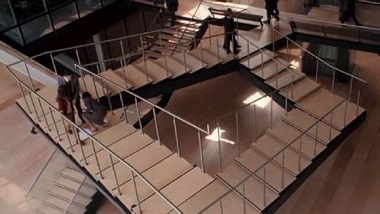
\includegraphics{rotation free.jpg}
    \end{center}
\par
 还有一些其他的例子可以表明这两个公式的作用:比如说,在电磁学里,高斯磁定律阐明,磁场的散度等于零(磁场线可以看成是一些闭合的磁场线,既然是闭合的,那就不存在起点和终点,则无源,即散度为零);在牛顿万有引力理论中,重力场就是梯度矢量场(保守场),因此重力场是无旋的。


\subsection{总结}
\begin{结论}{总结}
      梯梯度:(1)空间分布的不均匀程度;(2)沿空间变化最快的方向
      \par
      散度:单位体积的膨胀率
      \par
      旋度:单位体积内质点的旋转强度
      \par
      对任意n阶张量,做梯度之后的结果为(n+1)阶张量;对任意n阶张量做散度操作,结果为(n-1)阶张量。
      \par
      矢量场的分类:(1)螺管场——散度为零的矢量场;(2)无旋场——旋度为零的矢量场;(3)Laplacian 场:散度、旋度都为零。
\end{结论}
\end{document}